\documentclass{beamer}

\usepackage{qtree}
\usepackage{tikz}
\usepackage[UKenglish]{isodate}
\usetikzlibrary{mindmap,trees}
\usecolortheme{dove} 
\setbeamertemplate{navigation symbols}{}

\newcommand{\nonterm}[1]{$\left<#1\right>$}
\newcommand{\galt}[0]{$|$}

\begin{document}

\title{Introduction to Lambda Calculus}
\author{Maciek Makowski (@mmakowski)}

% -------------------------------------------
\frame{\titlepage}
% -------------------------------------------
\begin{frame}
\frametitle{The Plan}
\begin{center}
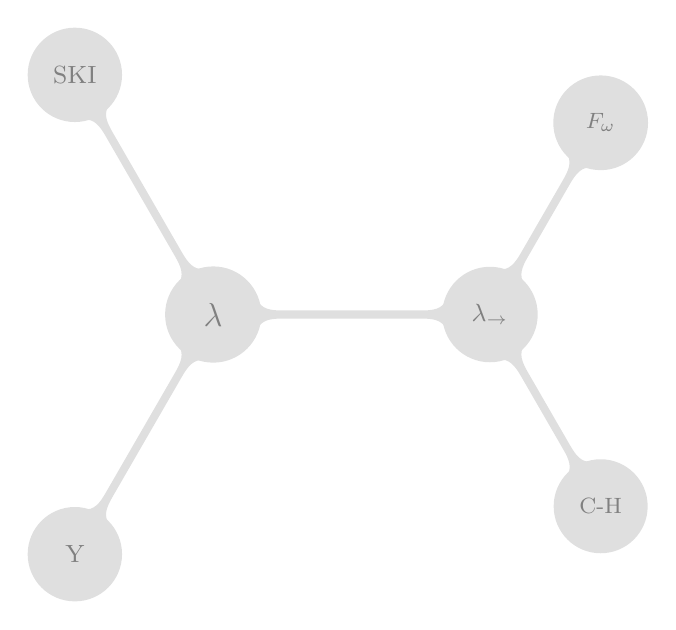
\begin{tikzpicture}
\path[mindmap, 
      concept color=lightgray!50!white,text=gray,
      every node/.style={minimum size=0pt,text width=30pt},
      level 1 concept/.append style={level distance=100,sibling angle=120},
      level 2 concept/.append style={level distance=80,sibling angle=120}
     ]
    node[concept] {$\lambda$}
    [clockwise from=0]
    child[concept] {
      node[concept] {$\lambda_\rightarrow$}
      [clockwise from=60]
      child { node[concept] {$F_\omega$} }
      child { node[concept] {C-H} }
    }  
    child[concept] { node[concept] {Y} }
    child[concept] { node[concept] {SKI} };
\end{tikzpicture}
\end{center}
\end{frame}
% -------------------------------------------
\begin{frame}
\frametitle{Basic Lambda Calculus}
\begin{center}
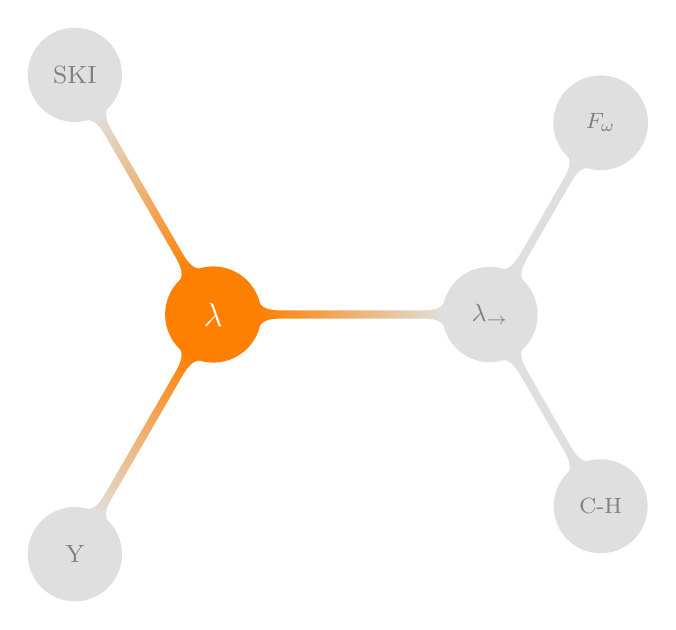
\begin{tikzpicture}
\path[mindmap, 
      concept color=orange,text=white,
      every node/.style={minimum size=0pt,text width=30pt},
      level 1 concept/.append style={level distance=100,sibling angle=120},
      level 2 concept/.append style={level distance=80,sibling angle=120}
     ]
    node[concept] {$\lambda$}
    [clockwise from=0]
    child[concept color=lightgray!50!white,text=gray] {
      node[concept] {$\lambda_\rightarrow$}
      [clockwise from=60]
      child { node[concept] {$F_\omega$} }
      child { node[concept] {C-H} }
    }  
    child[concept color=lightgray!50!white,text=gray] { node[concept] {Y} }
    child[concept color=lightgray!50!white,text=gray] { node[concept] {SKI} };
\end{tikzpicture}
\end{center}
\end{frame}
% -------------------------------------------
\begin{frame}
\frametitle{Syntax}
\begin{tabbing}
\nonterm{term} \= ::=  \= $x$~~~~~~~~~~~~~~~~~~~~~~~~~~~~  \= (variable)    \\
               \> \galt \> ($\lambda x.$\nonterm{term})    \> (abstraction) \\
               \> \galt \> (\nonterm{term} \nonterm{term}) \> (application) 
\end{tabbing}
where $x\in \mathbb{X}$ -- the set of variables

\end{frame}
% -------------------------------------------
\begin{frame}
\frametitle{Syntax}
\begin{tabbing}
~~~~~~~~~~~~~~~~~~~~~~~~~~~~~~~~~~ \= ~~~~~~~~~~~~~~~~~~~~~~~~~~~~~~~~~~~~ \\
$v_1$                              \>                                      \\
\end{tabbing}
\end{frame}
% -------------------------------------------
\begin{frame}
\frametitle{Syntax}
\begin{tabbing}
~~~~~~~~~~~~~~~~~~~~~~~~~~~~~~~~~~ \= ~~~~~~~~~~~~~~~~~~~~~~~~~~~~~~~~~~~~ \\
$v_1$                              \> \Tree [.{var $v_1$} ]                \\
\end{tabbing}
\end{frame}
% -------------------------------------------
\begin{frame}
\frametitle{Syntax}
\begin{tabbing}
~~~~~~~~~~~~~~~~~~~~~~~~~~~~~~~~~~ \= ~~~~~~~~~~~~~~~~~~~~~~~~~~~~~~~~~~~~ \\
$x\ y$                 \>                                      \\
\end{tabbing}
\end{frame}
% -------------------------------------------
\begin{frame}
\frametitle{Syntax}
\begin{tabbing}
~~~~~~~~~~~~~~~~~~~~~~~~~~~~~~~~~~ \= ~~~~~~~~~~~~~~~~~~~~~~~~~~~~~~~~~~~~ \\
$x\ y$                             \> \Tree [.app {var $x$} {var $y$} ]    \\
\end{tabbing}
\end{frame}
% -------------------------------------------
\begin{frame}
\frametitle{Syntax}
\begin{tabbing}
~~~~~~~~~~~~~~~~~~~~~~~~~~~~~~~~~~ \= ~~~~~~~~~~~~~~~~~~~~~~~~~~~~~~~~~~~~ \\
$\lambda a.b$                      \>                                      \\
\end{tabbing}
\end{frame}
% -------------------------------------------
\begin{frame}
\frametitle{Syntax}
\begin{tabbing}
~~~~~~~~~~~~~~~~~~~~~~~~~~~~~~~~~~ \= ~~~~~~~~~~~~~~~~~~~~~~~~~~~~~~~~~~~~ \\
$\lambda a.b$                      \> \Tree [.{abs $a$} {var $b$} ]        \\
\end{tabbing}
\end{frame}
% -------------------------------------------
\begin{frame}
\frametitle{Syntax}
\begin{tabbing}
~~~~~~~~~~~~~~~~~~~~~~~~~~~~~~~~~~ \= ~~~~~~~~~~~~~~~~~~~~~~~~~~~~~~~~~~~~ \\
$(\lambda a.\lambda b.a)\ c\ (\lambda b.b)$ \>                             \\
\end{tabbing}
\end{frame}
% -------------------------------------------
\begin{frame}
\frametitle{Syntax}
\begin{tabbing}
\nonterm{term} \= ::=  \= $x$~~~~~~~~~~~~~~~~~~~~~~~~~~~~  \= (variable)    \\
               \> \galt \> ($\lambda x.$\nonterm{term})    \> (abstraction) \\
               \> \galt \> (\nonterm{term} \nonterm{term}) \> (application) 
\end{tabbing}
\end{frame}
% -------------------------------------------
\begin{frame}
\frametitle{Syntax}
\begin{tabbing}
~~~~~~~~~~~~~~~~~~~~~~~~~~~~~~~~~~ \= ~~~~~~~~~~~~~~~~~~~~~~~~~~~~~~~~~~~~ \\
$(\lambda a.\lambda b.a)\ c\ (\lambda b.b)$ \> \Tree [.app [.app [.{abs $a$} 
[.{abs $b$} {var $a$} ] ] {var $c$} ] [.{abs $b$} {var $b$} ] ]             \\
\end{tabbing}
\end{frame}
% -------------------------------------------
\begin{frame}
\frametitle{Rewriting}
TODO
\end{frame}
% -------------------------------------------
\begin{frame}
\frametitle{Programming in Lambda Calculus}
\begin{center}
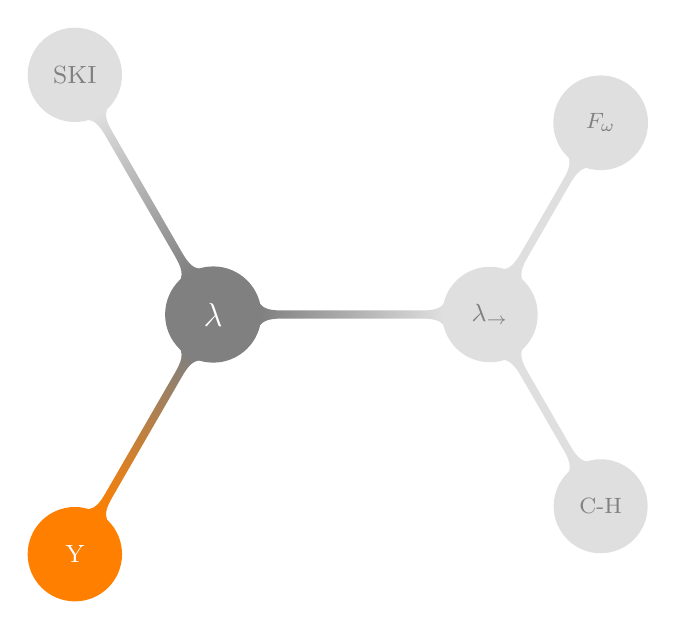
\begin{tikzpicture}
\path[mindmap, 
      concept color=gray,text=white,
      every node/.style={minimum size=0pt,text width=30pt},
      level 1 concept/.append style={level distance=100,sibling angle=120},
      level 2 concept/.append style={level distance=80,sibling angle=120}
     ]
    node[concept] {$\lambda$}
    [clockwise from=0]
    child[concept color=lightgray!50!white,text=gray] {
      node[concept] {$\lambda_\rightarrow$}
      [clockwise from=60]
      child { node[concept] {$F_\omega$} }
      child { node[concept] {C-H} }
    }  
    child[concept color=orange] { node[concept] {Y} }
    child[concept color=lightgray!50!white,text=gray] { node[concept] {SKI} };
\end{tikzpicture}
\end{center}
\end{frame}
% -------------------------------------------
\begin{frame}
\frametitle{Simple Types}
\begin{center}
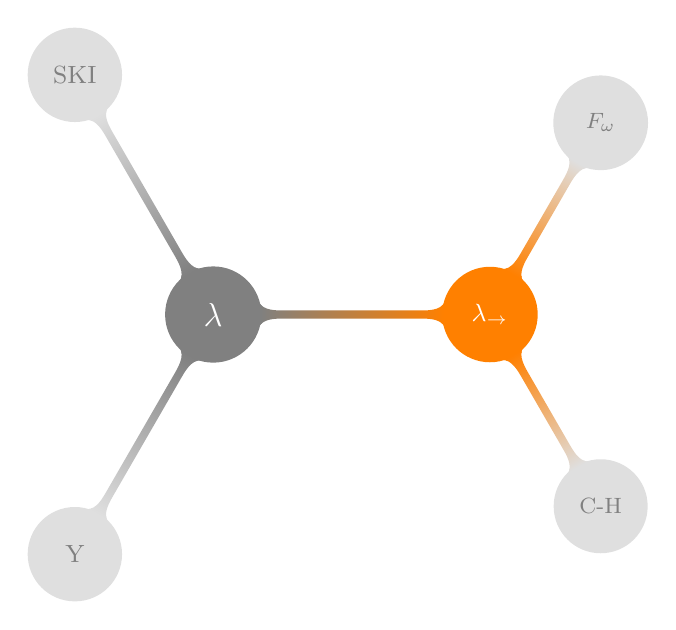
\begin{tikzpicture}
\path[mindmap, 
      concept color=gray,text=white,
      every node/.style={minimum size=0pt,text width=30pt},
      level 1 concept/.append style={level distance=100,sibling angle=120},
      level 2 concept/.append style={level distance=80,sibling angle=120}
     ]
    node[concept] {$\lambda$}
    [clockwise from=0]
    child[concept color=orange] {
      node[concept] {$\lambda_\rightarrow$}
      [clockwise from=60]
      child[concept color=lightgray!50!white,text=gray] { node[concept] {$F_\omega$} }
      child[concept color=lightgray!50!white,text=gray] { node[concept] {C-H} }
    }  
    child[concept color=lightgray!50!white,text=gray] { node[concept] {Y} }
    child[concept color=lightgray!50!white,text=gray] { node[concept] {SKI} };
\end{tikzpicture}
\end{center}
\end{frame}

\end{document}
